\documentclass[12pt,letterpaper]{article}
\usepackage[utf8]{inputenc}
\usepackage[spanish]{babel}
\usepackage{graphicx}
\usepackage[left=2cm,right=2cm,top=2cm,bottom=2cm]{geometry}
\usepackage{graphicx} % figuras
% \usepackage{subfigure} % subfiguras
\usepackage{float} % para usar [H]
\usepackage{amsmath}
%\usepackage{txfonts}
\usepackage{stackrel} 
\usepackage{multirow}
\usepackage{enumerate} % enumerados
\renewcommand{\labelitemi}{$-$}
\renewcommand{\labelitemii}{$\cdot$}
% \author{}
% \title{Caratula}
\begin{document}

% Fancy Header and Footer
% \usepackage{fancyhdr}
% \pagestyle{fancy}
% \cfoot{}
% \rfoot{\thepage}
%

% \usepackage[hidelinks]{hyperref} % CREA HYPERVINCULOS EN INDICE

% \author{}
\title{Caratula}

\begin{titlepage}
\begin{center}
\large{UNIVERSIDAD PRIVADA DE TACNA}\\
\vspace*{-0.025in}
\begin{figure}[htb]
\begin{center}

\includegraphics[width=7cm]{./images/logo}
\end{center}
\end{figure}
\vspace*{0.15in}
INGENIERIA DE SISTEMAS  \\

\vspace*{0.3in}
\begin{large}
\textbf{TITULO:} \\
\end{large}

\vspace*{0.1in}
\begin{Large}
\textbf{Informe de Laboratorio 05: Utilizando Desarrollo guiado por comportamiento (BDD)
para realización pruebas de software} \\

\end{Large}

\vspace*{0.3in}
\begin{Large}
\textbf{CURSO:} \\
\end{Large}

\vspace*{0.1in}
\begin{large}
Calidad y Pruebas de Software\\
\end{large}

\vspace*{0.3in}
\begin{Large}
\textbf{DOCENTE:} \\
\end{Large}

\vspace*{0.1in}
\begin{large}
 Ing. Patrick Cuadros Quiroga\\
\end{large}

\vspace*{0.4in}
\vspace*{0.1in}
\begin{large}
\textbf{INTEGRANTES:} \\
\begin{flushleft}
Yaneth Virginia Aquino Huallpa \hfill	(2017059286)\\

\centering  %CENTRA UN TEXTO
\vspace*{0.9in}
\begin{large}
Tacna
\end{large}

\end{flushleft}
\end{large}
\end{center}

\end{titlepage}





\section{Parte 1:Procedimiento} 
\begin{itemize}
 \item Se utilizará el framework CoreBDD. Instalar la plantilla de proyecto dotnet a través de
 dotnet new -i corebdd.projecttemplate
\begin{center}
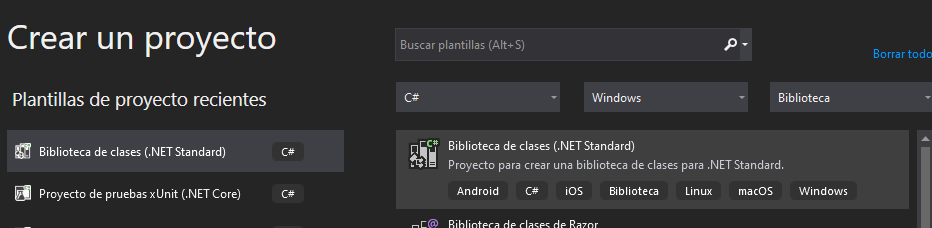
\includegraphics[width=\columnwidth]{images/1}\newline
\end{center}

\item Luego cree una nueva carpeta para su proyecto de prueba y ejecute
 dotnet new corebdd
\item Alternativamente, puede agregar CoreBDD a un proyecto de prueba xUnit existente a través del paquete
nuget
 dotnet add package CoreBDD
\begin{center}
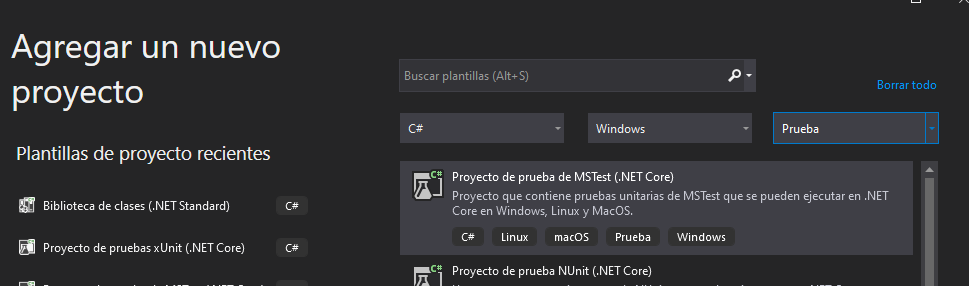
\includegraphics[width=\columnwidth]{images/2}\newline
\end{center}
\item También hay una herramienta de línea de comandos opcional para ejecutar pruebas con salida
personalizada, clases de prueba de andamios (características / escenarios / pasos) y generación de código
bidireccional (pruebas de Gherkin a CoreBDD y viceversa). Hay más documentación disponible sobre la CLI
en la parte inferior de esta página.
 dotnet tool install -g corebdd.commandline

\begin{center}
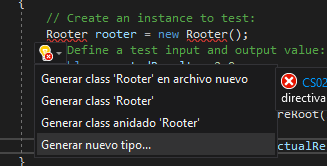
\includegraphics[width=\columnwidth]{images/3}\newline
\end{center}

\end{itemize}
\section{Escribir pruebas de CoreBDD} 
-----
\begin{itemize}
 \item Siguiendo el ejemplo habitual de la calculadora, podemos comenzar con el siguiente modelo para probar
\begin{center}
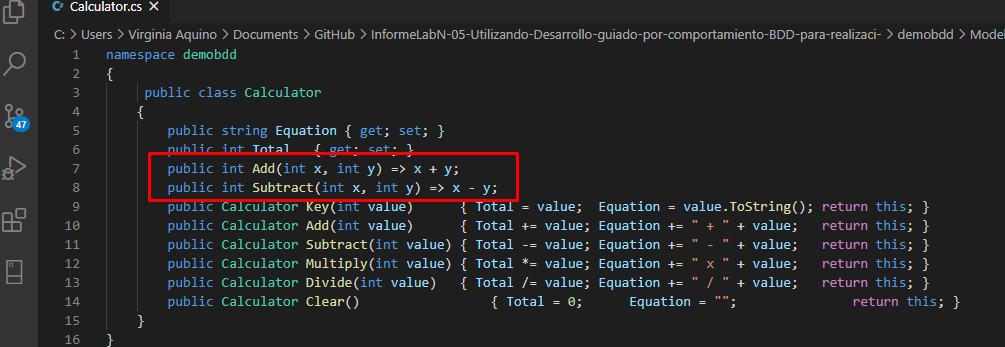
\includegraphics[width=\columnwidth]{images/001}\newline
\end{center}
\item Podemos definir una Característica para cotejar un conjunto de escenarios derivando de la clase
base Especificación y decorando con el atributo Característica. Tenga en cuenta que ambos constructores
son necesarios para admitir los diferentes estilos de sintaxis de prueba.
\begin{center}
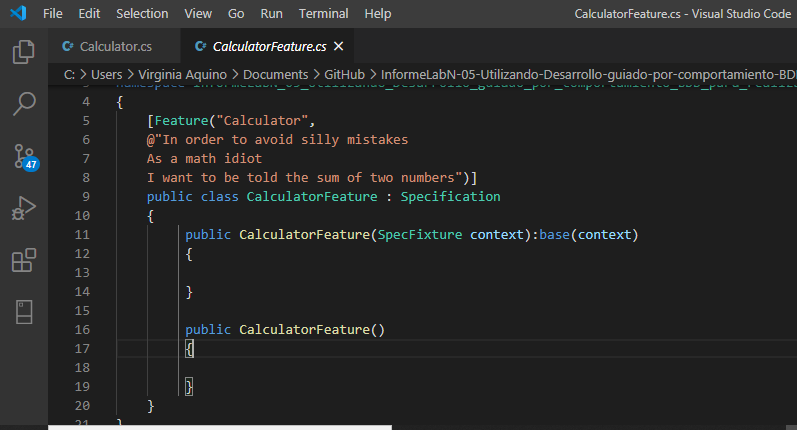
\includegraphics[width=\columnwidth]{images/002}\newline
\end{center}
\item Una vez que hemos creado nuestra Característica base, tenemos varios sabores diferentes para escribir
pruebas, primero podemos generar un escenario por clase (similar a las pruebas de estilo Cucumber) con
un método para cada paso de Dado / Cuándo / Entonces. Para hacer esto, simplemente herede de la
nueva clase de entidad, decore con un atributo de ejemplo y proporcione los métodos Given, When, Then
que se ejecutarán en orden
\begin{center}
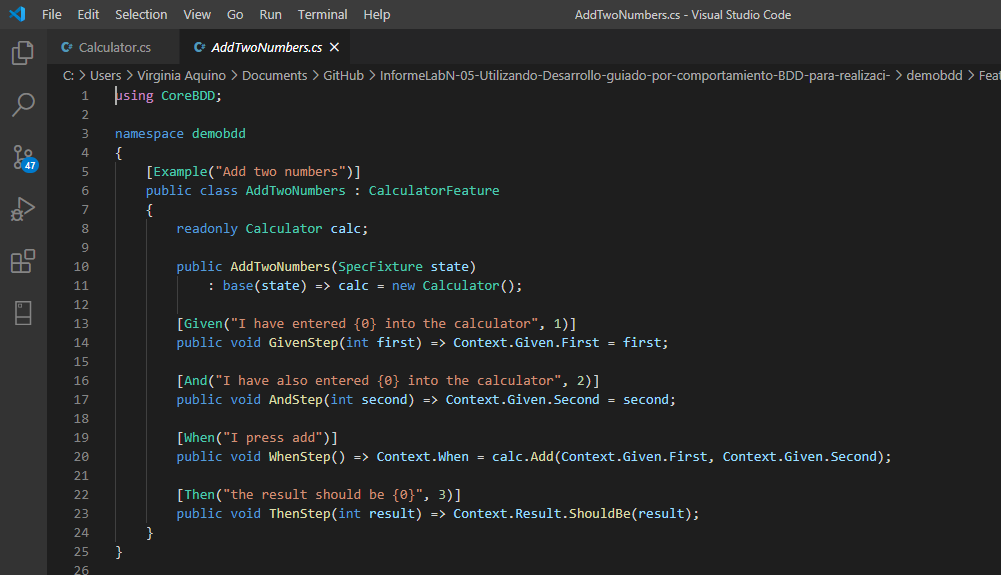
\includegraphics[width=\columnwidth]{images/003}\newline
\end{center}
\item También puede definir escenarios en un solo método utilizando delegados para cada uno de los pasos y
permitiendo que se definan múltiples escenarios dentro de la misma clase
\begin{center}
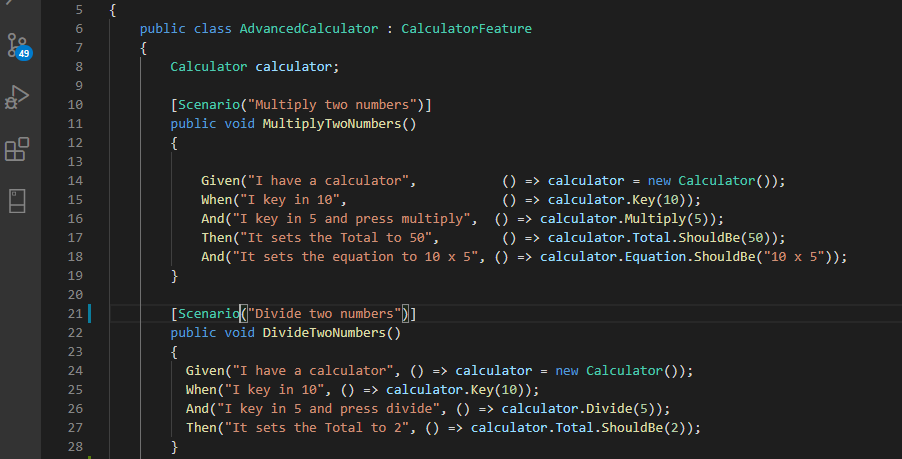
\includegraphics[width=\columnwidth]{images/004}\newline
\end{center}
\item La sintaxis basada en métodos también admite pruebas basadas en datos, utilizando xUnit InlineData (los
escenarios basados en clases aún no admiten pruebas basadas en datos).
\begin{center}
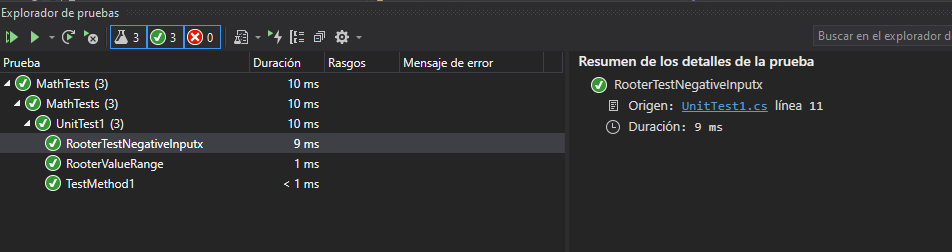
\includegraphics[width=\columnwidth]{images/005}\newline
\end{center}
\item Puede generar especificaciones de Gherkin de sus pruebas utilizando la biblioteca de
extensiones CoreBDD.SpecGeneration , ya sea llamando desde una aplicación o herramienta de línea de
comandos y pasando la ruta al ensamblado que contiene las pruebas, o conectando su proyecto de
prueba para generar las especificaciones después de prueba de funcionamiento.
Para hacer esto último, primero haga referencia a la biblioteca CoreBDD.SpecGeneration
\begin{center}
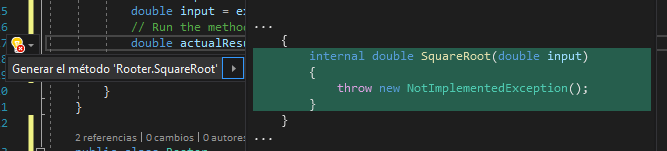
\includegraphics[width=\columnwidth]{images/5}\newline
\end{center}
\item A continuación, cree una clase de Fixture dentro de su proyecto de prueba y llame
a GenerateSpecs.OutputFeatureSpecs dentro del método Dispose, pasando el ensamblado (o ruta al
ensamblado) y la carpeta de salida para las especificaciones generadas.
\begin{center}
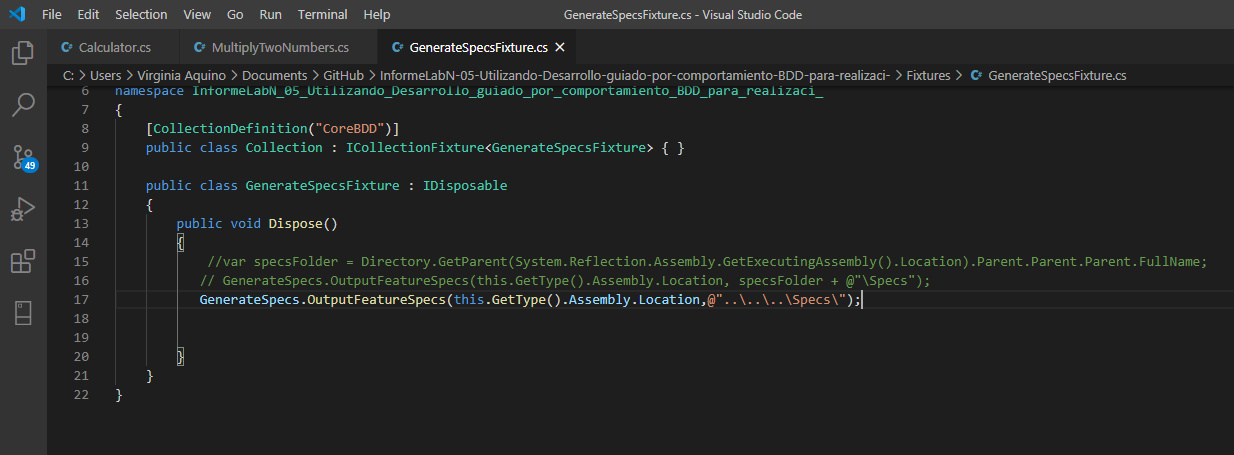
\includegraphics[width=\columnwidth]{images/006}\newline
\end{center}
\item Cuando las pruebas terminan de ejecutarse, se genera un archivo FeatureName.feature en la carpeta
Especificaciones del proyecto de prueba xUnit. Genera especificaciones de Gherkin para la característica y
los escenarios relacionados. Ejemplo CalculatorFeature.feature :
\begin{center}
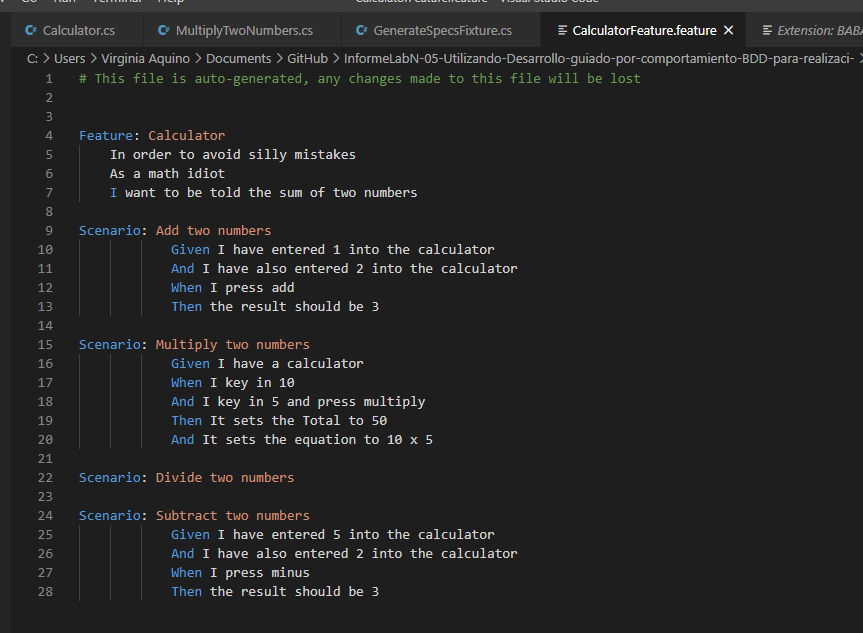
\includegraphics[width=\columnwidth]{images/007}\newline
\end{center}
\end{itemize}
\section{Herramienta de línea de comando} 
\begin{itemize}
\item La herramienta de línea de comandos facilita la ejecución de tareas como la ejecución de pruebas con la
salida de estilo Gherkin, la generación de archivos de prueba de características y escenarios
predeterminados y la generación de archivos de funciones de Gherkin a partir de pruebas existentes o la
generación de pruebas a partir de archivos de funciones existentes.
\item Comenzando desde cero usando la plantilla dotnet y las herramientas cli:
 mkdir demobdd
 cd demobdd
\item Luego cree el nuevo proyecto CoreBDD
 dotnet new corebdd
\item Encuentra pruebas de CoreBDD en directorios actuales y secundarios y ejecuta pruebas
\begin{center}
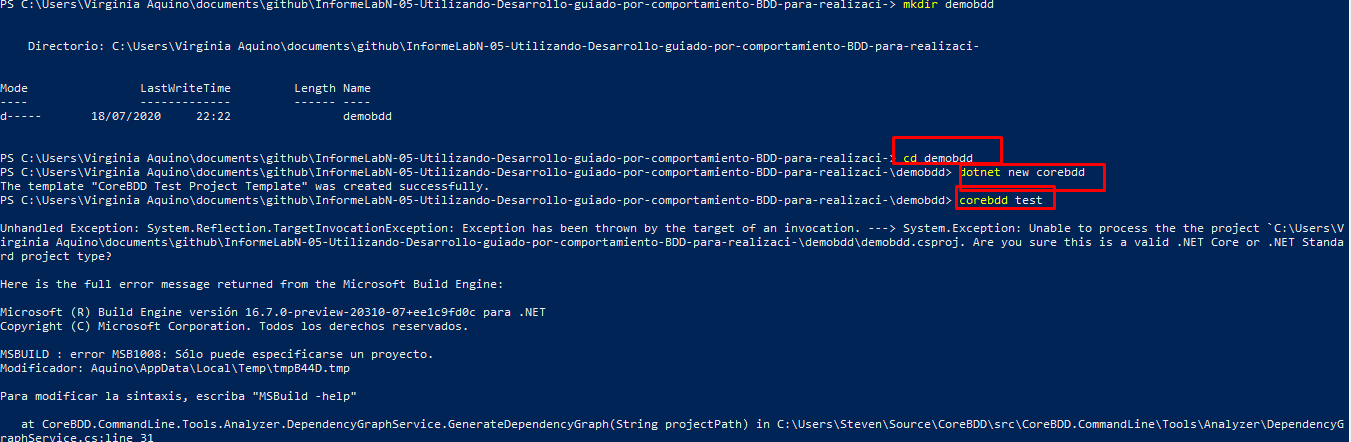
\includegraphics[width=\columnwidth]{images/6}\newline
\end{center}
\item Ejecute pruebas y luego genere archivos .feature de Gherkin en una ubicación específica
 corebdd test --specs --output ./Specs
\begin{center}
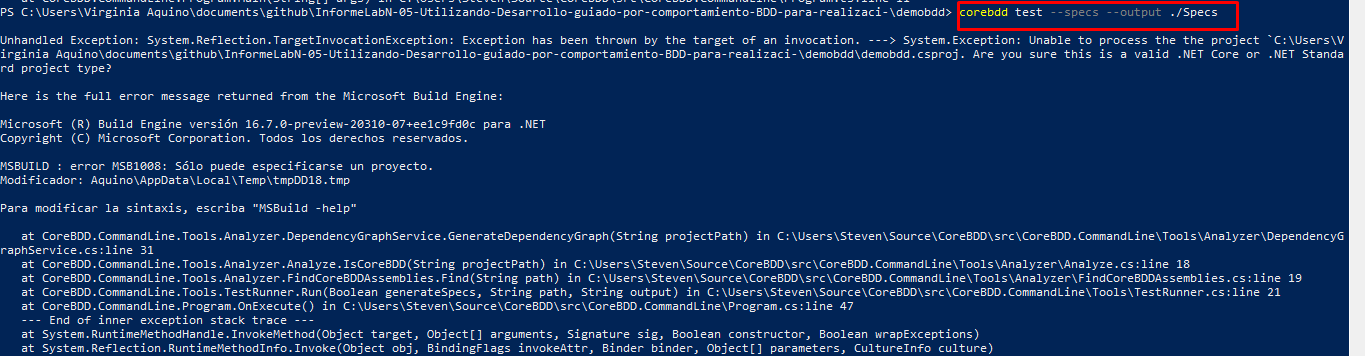
\includegraphics[width=\columnwidth]{images/7}\newline
\end{center}
\item Andamio de una clase de entidad CoreBDD llamada 'Iniciar sesión' en la carpeta actual
 corebdd generate feature --name login --namespace demobdd
\item Andamio de una clase de escenario CoreBDD llamada 'LoginToWebsite' en la función 'Iniciar sesión'
corebdd generate scenario --name LoginToWebsite --feature login --namespace demobdd
\begin{center}
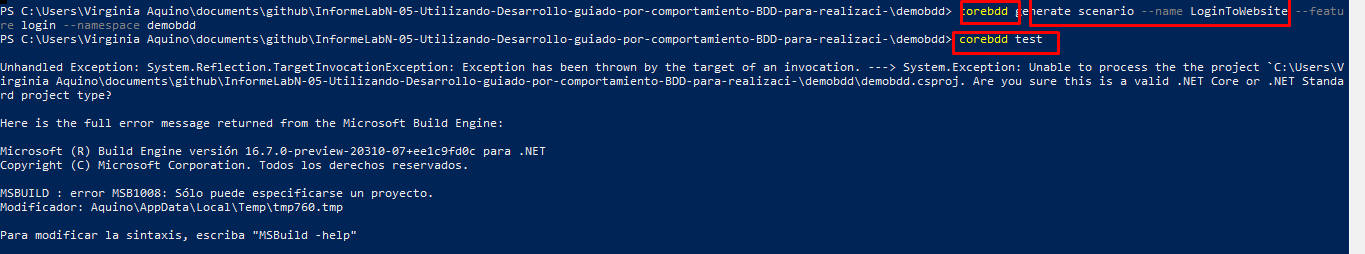
\includegraphics[width=\columnwidth]{images/8}\newline
\end{center}
\item Scaffold CoreBDD Pruebas de archivos existentes '.feature' de pepinillo, especificando la ubicación de los
archivos de características y la carpeta de destino para las pruebas generadas.
\item Si ha seguido utilizando el ejemplo de prueba 'corebdd', elimine la carpeta 'Características' (dejando la
carpeta Especificaciones con archivos .feature intactos) y luego ejecute:
corebdd generate tests --path ./Specs --output ./Features --namespace demobdd
\begin{center}
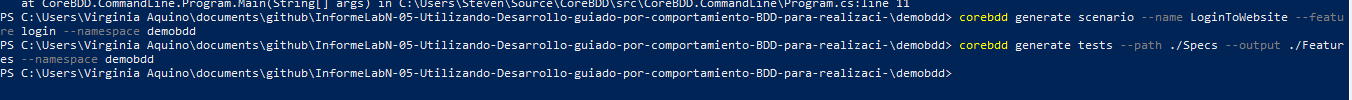
\includegraphics[width=\columnwidth]{images/9}\newline
\end{center}
\item Ahora debería tener los apéndices de prueba regenerados utilizando los escenarios de archivo .feature.
\begin{center}
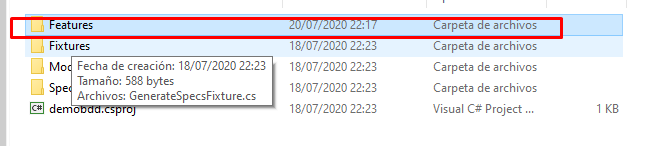
\includegraphics[width=\columnwidth]{images/10}\newline
\end{center}
\end{itemize}

\end{document}